% ============================================================
% GENERATED FILE — do not edit.
% Produced by tools/build-lesson-print.js from
% Space_Unit_Booklet_Yr7_8.tex. Edit the master and re-run:
%   node tools/build-lesson-print.js 1
% ============================================================
% ============================================================
%  Space — Unit Booklet
%  Years 7–8  |  Victorian Curriculum F–10 Version 2.0
%  Compile with: xelatex Space_Unit_Booklet_Yr7_8.tex  (twice for page refs)
%  Fonts: ./fonts/ — same folder as Forces and Bio booklets
% ============================================================
\documentclass[11pt,a4paper]{article}

% ── Fonts (compile with XeLaTeX) ─────────────────────────────────────────────
\usepackage{fontspec}
\setmainfont{Lato}[
  Path=./fonts/, Extension=.ttf, Ligatures=TeX,
  UprightFont=Lato-Regular, ItalicFont=Lato-Italic,
  BoldFont=Lato-Bold, BoldItalicFont=Lato-BoldItalic ]
\newfontfamily\headingfont{Poppins}[
  Path=./fonts/, Extension=.ttf, Ligatures=TeX,
  UprightFont=Poppins-Regular, ItalicFont=Poppins-Italic,
  BoldFont=Poppins-Bold, BoldItalicFont=Poppins-BoldItalic ]
\setlength{\headheight}{22pt}

\usepackage[protrusion=true,expansion=false]{microtype}
\usepackage[a4paper, top=2cm, bottom=2cm, left=2cm, right=2cm]{geometry}
\usepackage{xcolor}
\usepackage{tikz}
\usetikzlibrary{arrows.meta, shapes.geometric, calc, positioning,
                decorations.pathreplacing, backgrounds, patterns}
\usepackage{tcolorbox}
\tcbuselibrary{skins, breakable, raster}
\usepackage{fancyhdr}
\usepackage{titlesec}
\usepackage{enumitem}
\usepackage{booktabs}
\usepackage{tabularx}
\usepackage{array}
\usepackage{colortbl}
\usepackage{multicol}
\usepackage{amsmath}
\usepackage{needspace}
\usepackage{lastpage}
\usepackage{calc}
\usepackage{mdframed}
\usepackage{setspace}
\usepackage{ragged2e}
\usepackage{graphicx}
\usepackage{hyperref}
\usepackage{float}

% ── Colour Palette ───────────────────────────────────────────────────────────
% Primary: Space / Navy (unit identity)
\definecolor{Navy}       {HTML}{0B1A3E}
\definecolor{Space}      {HTML}{1B3378}
\definecolor{SpaceLight} {HTML}{E4E9F7}
\definecolor{SpaceMid}   {HTML}{2E4FAF}
% Gold accent
\definecolor{Gold}       {HTML}{D4A017}
\definecolor{GoldLight}  {HTML}{FBF3D5}
\definecolor{GoldDark}   {HTML}{C77F12}
% Supporting accents
\definecolor{Teal}       {HTML}{18A999}
\definecolor{TealLight}  {HTML}{E0F5F3}
\definecolor{Coral}      {HTML}{E8603C}
\definecolor{CoralLight} {HTML}{FDEEE9}
\definecolor{Violet}     {HTML}{7C4DBC}
\definecolor{VioletLight}{HTML}{F0EBF9}
% Earth / First Nations
\definecolor{Earth}      {HTML}{8B6340}
\definecolor{EarthDark}  {HTML}{5E3A1A}
\definecolor{EarthLight} {HTML}{F5EDE4}
% Neutrals
\definecolor{Ink}        {HTML}{16223A}
\definecolor{DarkGrey}   {HTML}{3A4759}
\definecolor{Grey}       {HTML}{5B6B82}   % secondary neutral; kept for body compatibility
\definecolor{MidGrey}    {HTML}{AEBED4}
\definecolor{LightGrey}  {HTML}{F2F5FA}
\definecolor{Line}       {HTML}{DDE5F0}
\definecolor{Paper}      {HTML}{FBFCFE}
% Table colours (Space-themed)
\definecolor{TableHead}  {HTML}{1B3378}
\definecolor{RowAlt}     {HTML}{E4E9F7}

% ── Hyperref ─────────────────────────────────────────────────────────────────
\hypersetup{
  colorlinks = true,
  linkcolor  = Space,
  urlcolor   = Teal,
  pdftitle   = {Space Unit Booklet --- Year 7/8 Science},
  pdfauthor  = {Northcote High School Science Department}
}

% ── Page Style ───────────────────────────────────────────────────────────────
\pagestyle{fancy}
\fancyhf{}
\renewcommand{\headrulewidth}{0.4pt}
\renewcommand{\headrule}{\hbox to\headwidth{\color{Space}\leaders\hrule height \headrulewidth\hfill}}
\fancyhead[L]{\headingfont\small\color{Space}Space}
\fancyhead[R]{\headingfont\small\color{DarkGrey}Years 7--8 \textbar{} Victorian Curriculum F--10 v2.0}
\fancyfoot[C]{\headingfont\small\color{DarkGrey}\thepage\ \textbar{} \pageref{LastPage}}
\fancypagestyle{plain}{%
  \fancyhf{}
  \fancyfoot[C]{\headingfont\small\color{DarkGrey}\thepage\ \textbar{} \pageref{LastPage}}
  \renewcommand{\headrulewidth}{0pt}
}

% ── Section Formatting ───────────────────────────────────────────────────────
\titleformat{\section}
  {\headingfont\color{Space}\Large\bfseries}
  {}{0em}{}
  [{\color{Teal}\rule[0.6ex]{2.2em}{3pt}}{\color{Line}\rule[0.6ex]{\dimexpr\linewidth-2.2em\relax}{1pt}}]
\titlespacing{\section}{0pt}{18pt}{8pt}

\titleformat{\subsection}
  {\headingfont\color{SpaceMid}\large\bfseries}
  {\thesubsection}{0.6em}{}
\titlespacing{\subsection}{0pt}{12pt}{4pt}

\titleformat{\subsubsection}
  {\headingfont\color{Space}\normalsize\bfseries}
  {}{0em}{}
\titlespacing{\subsubsection}{0pt}{8pt}{2pt}

% Deck-style eyebrow / kicker
\newcommand{\kicker}[2][Teal]{%
  {\headingfont\bfseries\footnotesize\color{#1}%
   \textcolor{#1}{\rule[0.18ex]{1.6em}{2.2pt}}\hspace{0.5em}\MakeUppercase{#2}\par}%
  \vspace{2pt}}

% ── Custom tcolorbox Environments ────────────────────────────────────────────

% Section divider banner (navy)
\newcommand{\sectiondiv}[3]{%
  \needspace{5\baselineskip}
  \begin{tcolorbox}[
    enhanced, breakable=false, arc=3.5mm,
    colback=Navy, colframe=Navy, boxrule=0pt,
    sidebyside, sidebyside align=center,
    lefthand width=2.0cm,
    left=2mm, right=4mm, top=4mm, bottom=4mm
  ]
    \begin{center}
      {\headingfont\bfseries\color{white!35!Navy}\fontsize{50}{50}\selectfont #1}
    \end{center}
    \tcblower
    {\headingfont\bfseries\color{white}\LARGE #2}\\[3pt]
    {\itshape\color{white!75!Navy}\small #3}
  \end{tcolorbox}%
}

% Key info box (space blue)
\newtcolorbox{infobox}[1]{
  breakable, arc=2.5mm, boxrule=0.5pt,
  colback=SpaceLight, colframe=Space!40,
  fonttitle=\headingfont\bfseries, coltitle=Space,
  title={#1},
  left=4mm, right=3.5mm, top=2.5mm, bottom=2.5mm
}

% First Nations callout (earth brown)
\newtcolorbox{fnbox}[1]{
  breakable, arc=2.5mm, boxrule=0.5pt,
  colback=EarthLight, colframe=Earth!40,
  fonttitle=\headingfont\bfseries, coltitle=EarthDark,
  title={#1},
  left=4mm, right=3.5mm, top=2.5mm, bottom=2.5mm
}

% Scaffold box (gold — structured student support, matches Forces/Bio)
\newtcolorbox{scaffold}[1]{
  breakable, arc=2.5mm, boxrule=0.5pt,
  colback=GoldLight, colframe=Gold!40,
  fonttitle=\headingfont\bfseries, coltitle=GoldDark,
  title={#1},
  left=4mm, right=3.5mm, top=2.5mm, bottom=2.5mm
}

% Worked example box (white bg, gold frame — matches Forces/Bio)
\newtcolorbox{workedex}[1]{
  breakable, arc=2.5mm, boxrule=0.5pt,
  colback=white, colframe=Gold!50,
  fonttitle=\headingfont\bfseries, coltitle=GoldDark,
  title={#1},
  left=4mm, right=3.5mm, top=2.5mm, bottom=2.5mm
}

% Year 7 box (space blue)
\newtcolorbox{yr7box}{
  breakable, arc=2.5mm, boxrule=0.5pt,
  colback=SpaceLight, colframe=Space!40,
  left=4mm, right=3.5mm, top=2.5mm, bottom=2.5mm
}

% Year 8 extension box (violet — same across all units)
\newtcolorbox{yr8box}{
  breakable, arc=2.5mm, boxrule=0.5pt,
  colback=VioletLight, colframe=Violet!40,
  left=4mm, right=3.5mm, top=2.5mm, bottom=2.5mm
}

% Above-level banner for a whole section. Sits straight under the
% \section heading of a section that runs past the Year 7 level, and
% reuses the violet of yr8box so "violet = above the level" holds
% throughout the booklet. Not breakable — it is two or three lines.
\newtcolorbox{extbox}{
  breakable=false, arc=2.5mm, boxrule=0.9pt,
  colback=VioletLight, colframe=Violet!65,
  left=4mm, right=3.5mm, top=2.5mm, bottom=2.5mm
}
% Fill-in table rows. Entry-task tables are written in, so their rows need
% far more height than a reference table's. Wrap the tabular in
% \begin{fillin}...\end{fillin} rather than setting \arraystretch by hand,
% so every entry task in the booklet writes on the same size line.
\newenvironment{fillin}[1][2.6]{\begingroup\renewcommand{\arraystretch}{#1}}{\endgroup}

\newcommand{\extension}[1]{%
  \begin{extbox}
  {\headingfont\bfseries\color{Violet}Above level --- extension.}\ #1
  \end{extbox}
  \medskip
}

% ── Custom Commands ───────────────────────────────────────────────────────────

% Answer box: \answerbox{height e.g. 3cm}
% Drawing / working space: \answerbox{height}
%
% Deliberately NOT breakable — a fixed-height drawing box split across a
% page break is useless, and it is nested inside scaffold/yr7box, which
% are themselves breakable (tcolorbox does not support that combination).
% \needspace instead pushes the whole box to the next page if it will not
% fit. White rather than Paper so it matches the \anslines writing bands.
\newcommand{\answerbox}[1]{%
  \par\needspace{#1}%
  \begin{tcolorbox}[
    enhanced, breakable=false, arc=2mm,
    colback=white, colframe=Line,
    left=2mm, right=2mm, top=1mm, bottom=1mm,
    boxrule=1pt, height=#1
  ]
  \end{tcolorbox}%
}

% Question: \question{marks}{text}  (marks can be empty)
%
% Numbered automatically as Q<section>.<n>. The counter resets at every
% \section, so questions renumber themselves when content is inserted,
% deleted or reordered — do NOT write numbers by hand. \refstepcounter
% also means a \label right after a \question can be \ref'd elsewhere.
\newcounter{qnum}[section]
\renewcommand{\theqnum}{\thesection.\arabic{qnum}}
\newcommand{\question}[2]{%
  \refstepcounter{qnum}%
  \needspace{3\baselineskip}%
  \medskip
  \noindent\textbf{Q\theqnum}\ifx&#1&\else\ \textcolor{DarkGrey}{(#1 mark\ifnum#1=1\else s\fi)}\fi\quad #2%
  \medskip
}

% Inline marks note
\newcommand{\markscount}[1]{\hfill\textcolor{DarkGrey}{\textit{(#1 mark\ifnum#1=1\else s\fi)}}}

% Figure caption
\newcommand{\figcap}[1]{%
  \begin{center}\small\itshape\color{DarkGrey} #1\end{center}%
}

% Answer lines: \anslines{n}
%
% Each line is a white writing band with the rule drawn under it, so the
% writing area stays white inside the tinted yr7box/yr8box panels. Built
% one line at a time rather than as a single enclosing box because
% \anslines is used inside breakable tcolorboxes, and tcolorbox does not
% support nesting a breakable box inside another — this way a page break
% can fall between two lines quite happily.
%
% \anslineband is the pitch: keep it equal to the old \vspace so the
% writing space per line is unchanged.
\newlength{\anslineband}
\setlength{\anslineband}{\dimexpr\baselineskip+13pt\relax}
\newcommand{\anslines}[1]{%
  \par\vspace{2pt}%
  \begingroup
  \setlength{\fboxsep}{0pt}\setlength{\parskip}{0pt}%
  \foreach \n in {1,...,#1}{%
    \noindent\colorbox{white}{\makebox[\linewidth][l]{\rule{0pt}{\anslineband}}}\par\nointerlineskip
    \noindent\rule{\linewidth}{0.3pt}\par\nointerlineskip
  }%
  \endgroup
  \vspace{2pt}%
}

% Table column types
\newcolumntype{L}[1]{>{\RaggedRight\arraybackslash}p{#1}}
\newcolumntype{C}[1]{>{\Centering\arraybackslash}p{#1}}

% Table helpers
\newcommand{\thead}[1]{\cellcolor{TableHead}\color{white}\bfseries #1}
\newcommand{\talt}{\rowcolor{RowAlt}}
\newcommand{\tmid}{\rowcolor{MidGrey}}

% Vocabulary term
\newcommand{\vocab}[1]{\textbf{\textcolor{Space}{#1}}}

% Victorian Curriculum reference
\newcommand{\vc}[2]{\small\textcolor{DarkGrey}{\textit{VC 2.0: #1 --- #2}}}

\definecolor{moonshadow}{HTML}{2E3350} % --accent      (unlit)
\definecolor{moonlit}{HTML}{DCE6F5}    % --c-line-cool (lit)
\definecolor{moonink}{HTML}{1B1F2A}    % --ink
\definecolor{moonsoft}{HTML}{6B7280}   % --ink-soft

\newcommand{\moonR}{0.55}   % disc radius (cm)
\newcommand{\moonGap}{1.71} % centre spacing (cm) — SVG's 112/36 ratio

% {index}{mirror: 1=waxing, -1=waning}{terminator x-radius / R}{label}
\newcommand{\moonphase}[4]{%
	\begin{scope}[shift={(#1*\moonGap,0)}]
		\fill[moonshadow] (0,0) circle[radius=\moonR cm];
		\begin{scope}[xscale=#2]
			\fill[moonlit] (0,\moonR)
			arc[start angle=90,  end angle=-90, radius=\moonR cm]
			arc[start angle=-90, end angle=90,  x radius=#3*\moonR cm,
			y radius=\moonR cm] -- cycle;
		\end{scope}
		\draw[moonshadow, line width=0.4pt] (0,0) circle[radius=\moonR cm];
		\node[moonink, font=\scriptsize, align=center, anchor=north]
		at (0,-\moonR-0.14) {#4};
\end{scope}}

\usetikzlibrary{arrows.meta}

\definecolor{tideaccent}{HTML}{2E3350}   % --accent
\definecolor{tidewarm}{HTML}{C86A2E}     % --accent-warm
\definecolor{tidewarmsoft}{HTML}{FBE7D2} % --accent-warm-soft
\definecolor{tidecool}{HTML}{DCE6F5}     % --c-line-cool
\definecolor{tidefaint}{HTML}{9AA3B2}    % --ink-faint
\definecolor{tidesoft}{HTML}{6B7280}     % --ink-soft

% Coordinates below are the SVG's own (0,0)-(380,200) grid.
% 0.021cm per SVG unit  ->  the figure is 8 cm wide; change it to rescale.
\newcommand{\tideunit}{0.021cm}

% ============================================================
\begin{document}

% Compact single-lesson cover. The master booklet uses a full-bleed
% Navy titlepage; a handful of stapled sheets does not need one, and a
% full-page ink flood is unkind to a school printer.
\thispagestyle{fancy}
\begin{center}
  {\headingfont\small\color{Gold}NORTHCOTE HIGH SCHOOL\ \textbullet\ YEAR 7/8 SCIENCE\ \textbullet\ VICTORIAN CURRICULUM 2.0}\\[0.5em]
  {\headingfont\fontsize{26pt}{30pt}\selectfont\bfseries\color{Space}Space}\\[0.35em]
  {\headingfont\large\color{SpaceMid}Lesson 1 \textbullet\ Earth, Moon and Sun --- Scale and Structure}\\[0.7em]
  {\color{Gold}\rule{0.5\linewidth}{1.2pt}}\\[0.7em]
  \begin{minipage}{0.8\linewidth}\centering\small
    \textcolor{DarkGrey}{This is Section~1 of the Space unit booklet, printed on its own.
    Question numbers match the full booklet, so answers can be marked against the same key.}
  \end{minipage}\\[1.2em]
  \begin{minipage}{0.8\linewidth}
    \small\textbf{Name:}\ \rule{5cm}{0.4pt}\hfill\textbf{Class:}\ \rule{3cm}{0.4pt}
  \end{minipage}
\end{center}
\vspace{1.2em}

\setcounter{section}{0}

% ============================================================
\section{Earth, Moon and Sun --- Scale and Structure}
% ============================================================
\vc{Science Understanding}{Physical sciences: Earth and space sciences; scale and relative size of Earth, Moon and Sun}

\subsection{The scale of Earth, Moon and Sun}

The three most important objects in our immediate cosmic environment differ enormously in size. Understanding their relative sizes is foundational to everything else in this unit.

\begin{center}
\begin{tabular}{lrrr}
\toprule
\headingfont\textbf{Object} & \headingfont\textbf{Diameter (km)} & \headingfont\textbf{Mass (kg)} & \headingfont\textbf{Distance from Earth} \\
\midrule
Moon    & 3,474          & $7.34\times10^{22}$  & 384,400 km avg \\
Earth   & 12,742         & $5.97\times10^{24}$  & ---             \\
Sun     & 1,392,000      & $1.99\times10^{30}$  & 150,000,000 km (1 AU) \\
\bottomrule
\end{tabular}
\end{center}

\begin{infobox}{Key concept: Scale}
If Earth were the size of a tennis ball (6.7 cm across), the Moon would be a marble (1.8 cm) about 1.9 m away, and the Sun would be a sphere 7.5 m across, placed 807 m down the road. The solar system is almost entirely \vocab{empty space}.
\end{infobox}


\begin{yr7box}
\textbf{\headingfont Check your understanding}\hfill\textcolor{DarkGrey}{\itshape 8 marks}

\question{2}{Use the table to state the diameter of Earth and the diameter of the Sun.}
\anslines{2}

\question{2}{Calculate how many times wider the Sun is than Earth. Show your working and give your answer to the nearest whole number.}
\anslines{3}

\question{2}{The Moon is 384,400 km from Earth. Calculate how many Earth diameters would fit into that gap.}
\anslines{3}

\question{2}{In the tennis-ball model, Earth is 6.7 cm across and the Sun sits 807 m down the road. Explain what this model shows that the table of diameters alone does not.}
\anslines{3}

\end{yr7box}
\newpage
\subsection{Structure of Earth}

Earth has four main layers:
\begin{itemize}
  \item \vocab{Inner core} --- solid iron-nickel; radius ~1,200 km; temperature ~5,400°C
  \item \vocab{Outer core} --- liquid iron-nickel; generates Earth's magnetic field (the dynamo effect)
  \item \vocab{Mantle} --- semi-solid rock; 2,900 km thick; convection currents drive plate tectonics
  \item \vocab{Crust} --- thin, solid rock; 5--70 km thick; oceanic (denser, thinner) and continental (less dense, thicker)
\end{itemize}

\subsubsection{Diagram: Label the layers of Earth}
% Colours and band order mirror the slide-deck version of this diagram
% (deck1.html): the two outer layers in Space blue, the two core layers
% in Gold. Leader lines run out to a common rail on the right so the
% labels sit in a single column and cannot collide.
\begin{center}
\begin{tikzpicture}[
    band/.style={draw=white, line width=1.1pt},
    lead/.style={draw=black, line width=0.6pt, -{Stealth[length=4.5pt,width=3.5pt]}},
    ansrule/.style={right, inner sep=2pt}
  ]
  \filldraw[band, fill=Space!30] (0,0) circle (3.5cm);
  \filldraw[band, fill=Space!55] (0,0) circle (3.15cm);
  \filldraw[band, fill=Gold!45]  (0,0) circle (1.75cm);
  \filldraw[band, fill=Gold!90]  (0,0) circle (0.85cm);

  % arrowheads land inside the band being labelled
  \draw[lead] (4.25,3.25)  -- (1.70,2.8);
  \draw[lead] (4.25,1.95)  -- (1.95,1.5);
  \draw[lead] (4.25,0.60)  -- (1.30,0.72);
  \draw[lead] (4.25,-0.80) -- (0.50,-0.30);

  \node[ansrule] at (4.3,3.25)  {\rule{3.2cm}{0.5pt}};
  \node[ansrule] at (4.3,1.95)  {\rule{3.2cm}{0.5pt}};
  \node[ansrule] at (4.3,0.60)  {\rule{3.2cm}{0.5pt}};
  \node[ansrule] at (4.3,-0.80) {\rule{3.2cm}{0.5pt}};
\end{tikzpicture}

\vspace{0.6em}
{\small\textit{Word bank:}\quad Outer core \ \textbullet\ Crust \ \textbullet\ Inner core \ \textbullet\ Mantle}
\end{center}


\begin{yr7box}
\textbf{\headingfont Check your understanding}\hfill\textcolor{DarkGrey}{\itshape 8 marks}


\question{2}{Which layer generates Earth's magnetic field, and what is this process called?}
\anslines{2}

\question{2}{The mantle is described as semi-solid rock. State its thickness and what its convection currents drive.}
\anslines{2}

\question{2}{Compare oceanic and continental crust using two differences given in the booklet.}
\anslines{3}

\end{yr7box}


\newpage
\subsection{The Moon}

The Moon is Earth's only natural \vocab{satellite}. It produces no light of its own --- everything we see is reflected sunlight.

\begin{itemize}
  \item \textbf{Diameter}: 3,474 km --- about one quarter of Earth's
  \item \textbf{Distance}: 384,400 km from Earth on average; light crosses this in \textbf{1.28 seconds}
  \item \textbf{Orbital period}: 27.3 days --- and it \textit{rotates} in exactly the same time
  \item \textbf{Surface}: covered in \vocab{regolith}, a fine powdery rock produced by billions of years of meteorite impacts
  \item \textbf{No atmosphere} and no liquid water, so temperatures swing from $-173$\,°C at night to $+127$\,°C in daylight
\end{itemize}

\begin{infobox}{Why we only ever see one side}
The Moon's rotation period and orbital period are identical (27.3 days), so the same face is always turned towards Earth. This is called \vocab{tidal locking}, and it is the normal outcome for a moon orbiting close to a much larger body. The hemisphere we never see from Earth is the \textbf{far side} --- not the ``dark side.'' It receives just as much sunlight as the near side.
\end{infobox}

Two kinds of terrain are visible with the naked eye. The number of craters on a surface tells you how old it is: the longer a surface has been there, the more impacts it has collected.

\begin{itemize}
  \item \vocab{Highlands} --- the bright, rugged regions. This is the Moon's \textbf{original crust}, so it is the oldest surface. It has been exposed to meteorite impacts for the whole history of the Moon, which is why it is so heavily cratered
  \item \vocab{Maria} (singular \textit{mare}, Latin for ``sea'') --- the dark, flat plains. Later, huge impacts punched basins into the crust, and lava welled up and flooded them. When that lava cooled it created a \textbf{new, smooth surface}, wiping out the craters that were there before. Because this happened after the highlands formed, the maria have had less time to collect impacts --- so they are only lightly cratered
\end{itemize}


\begin{yr7box}
\textbf{\headingfont Check your understanding}\hfill\textcolor{DarkGrey}{\itshape 9 marks}

\question{3}{Explain why we always see the same face of the Moon from Earth.}
\anslines{3}

\question{2}{Describe the difference between the maria and the highlands, and state which is older.}
\anslines{3}

\question{2}{The Moon has no atmosphere. Explain how this causes its extreme temperature range.}
\anslines{3}

\end{yr7box}



\subsection{Structure of the Sun}

The Sun is a \vocab{main sequence star} --- it converts hydrogen into helium through \vocab{nuclear fusion} in its core.

\begin{itemize}
  \item \textbf{Core}: where fusion occurs; temperature ~15 million°C
  \item \textbf{Radiative zone}: energy moves outward as photons (takes ~100,000 years to cross)
  \item \textbf{Convective zone}: energy carried by convecting plasma
  \item \textbf{Photosphere}: the visible surface (~5,778 K); where sunspots form
  \item \textbf{Chromosphere and Corona}: outer atmosphere; much hotter than photosphere (corona: 1--3 million K)
\end{itemize}

\subsubsection{Diagram: Label the layers of the Sun}
% Same construction as the Earth diagram in 1.2.1 — concentric bands,
% white separators, leader lines out to a common rail on the right.
% Warm palette here rather than Space blue: gold ramp for the interior,
% Coral for the fusion core and the chromosphere.
\begin{center}
\begin{tikzpicture}[
    band/.style={draw=white, line width=1.1pt},
    lead/.style={draw=black, line width=0.6pt, -{Stealth[length=4.5pt,width=3.5pt]}},
    ansrule/.style={right, inner sep=2pt}
  ]
  \filldraw[band, fill=Gold!15]     (0,0) circle (3.60cm);
  \filldraw[band, fill=Coral!45]    (0,0) circle (3.22cm);
  \filldraw[band, fill=GoldDark!75] (0,0) circle (3.00cm);
  \filldraw[band, fill=Gold!40]     (0,0) circle (2.72cm);
  \filldraw[band, fill=Gold!70]     (0,0) circle (1.90cm);
  \filldraw[band, fill=Coral!90]    (0,0) circle (0.95cm);

  \draw[lead] (4.30,3.40)  -- (1.05,3.23);
  \draw[lead] (4.30,2.40)  -- (1.51,2.72);
  \draw[lead] (4.30,1.40)  -- (1.95,2.09);
  \draw[lead] (4.30,0.40)  -- (2.02,1.12);
  \draw[lead] (4.30,-0.60) -- (1.40,0.22);
  \draw[lead] (4.30,-1.60) -- (0.43,-0.25);

  \node[ansrule] at (4.35,3.40)  {\rule{3.2cm}{0.5pt}};
  \node[ansrule] at (4.35,2.40)  {\rule{3.2cm}{0.5pt}};
  \node[ansrule] at (4.35,1.40)  {\rule{3.2cm}{0.5pt}};
  \node[ansrule] at (4.35,0.40)  {\rule{3.2cm}{0.5pt}};
  \node[ansrule] at (4.35,-0.60) {\rule{3.2cm}{0.5pt}};
  \node[ansrule] at (4.35,-1.60) {\rule{3.2cm}{0.5pt}};
\end{tikzpicture}

\vspace{0.6em}
{\small\textit{Word bank:}\quad Convective zone \ \textbullet\ Corona \ \textbullet\ Core \ \textbullet\ Photosphere \ \textbullet\ Chromosphere \ \textbullet\ Radiative zone}
\end{center}

\begin{workedex}{Worked example: Light travel time from the Sun}
\textit{The Sun is 150,000,000 km from Earth. Light travels at 300,000 km/s. How long does sunlight take to reach us?}

\medskip
$\text{Time} = \dfrac{\text{Distance}}{\text{Speed}} = \dfrac{150{,}000{,}000 \text{ km}}{300{,}000 \text{ km/s}} = 500 \text{ s} = 8 \text{ min } 20 \text{ s}$

\medskip
\textbf{Answer}: Sunlight takes 8 minutes and 20 seconds to reach Earth. This means the Sun we see right now is actually how it looked 8 minutes ago.
\end{workedex}

\begin{scaffold}{Your turn}
A flash of light leaves the Moon. How long before we see it? (Moon is 384,400 km away; speed of light = 300,000 km/s)

\answerbox{4cm}
\end{scaffold}

% ============================================================
\newpage
\begin{yr7box}
\textbf{\headingfont Check your understanding}\hfill\textcolor{DarkGrey}{\itshape 9 marks}

\question{2}{Define nuclear fusion as it occurs in the Sun.}
\anslines{4}

\question{2}{State the temperature of the Sun's core and of its photosphere.}
\anslines{4}

\question{3}{Jupiter is 5.20 AU from the Sun. Sunlight reaches Earth (1 AU) in 500 seconds. Calculate how long sunlight takes to reach Jupiter, in minutes and seconds.}
\anslines{8}

\end{yr7box}
\newpage
\begin{yr8box}
	\textbf{Year 8 Extension: How the Moon formed --- the Giant Impact Hypothesis}
	
	The leading model for the Moon's origin is the \vocab{Giant Impact Hypothesis}. About \textbf{4.5 billion years ago} a Mars-sized body --- named \textbf{Theia} --- struck the young Earth. The collision threw a disc of molten rock and vapour into orbit, and that material clumped together under gravity to form the Moon.
	
	\medskip
	Two pieces of evidence support it:
	\begin{itemize}
		\item The Moon has almost \textbf{no iron core}. Earth's iron had already sunk to its centre before the impact, so the debris blasted into orbit came mostly from the rocky mantle.
		\item Moon rock returned by the Apollo missions has \textbf{oxygen isotope ratios identical to Earth's}. Rock formed elsewhere in the solar system does not match --- so the Moon and Earth are made of the same material.
	\end{itemize}
	
	\medskip
	\textbf{Why it matters}: the Moon's mass stabilises Earth's axial tilt at about 23.5°. Without it, the tilt could wander between 0° and 85° over millions of years, making stable long-term climates --- and possibly complex life --- far less likely.
\end{yr8box}

\begin{yr8box}
	\textbf{Year 8 Extension: Earth's magnetosphere and space weather}
	
	The liquid iron in Earth's \textbf{outer core} is constantly moving, and moving
	metal generates a magnetic field --- the \vocab{dynamo effect}. That field does
	not stop at the surface. It reaches tens of thousands of kilometres out into
	space, forming the \vocab{magnetosphere}: an invisible shield around the whole
	planet.
	
	\smallskip
	It has something to shield us from.
	
	\begin{itemize}
		\item \vocab{Solar wind} --- a constant stream of charged particles blowing
		outward from the Sun at 400--800 km/s. It never stops.
		\item \vocab{Coronal mass ejections} (CMEs) --- huge bursts of plasma thrown
		off the Sun, which can reach Earth in one to three days.
		\item \vocab{Auroras} --- the magnetosphere funnels charged particles toward
		the poles, where they collide with atmospheric gases and make them glow.
		This is the \textit{aurora australis} in the south and the
		\textit{aurora borealis} in the north. An aurora is what the shield
		looks like while it is working.
	\end{itemize}
	
	\smallskip
	\vocab{Space weather} is the name for these events, and it has consequences on
	the ground. On 13 March 1989 a geomagnetic storm induced currents in Quebec's
	power transmission lines large enough to collapse the entire provincial grid in
	under 90 seconds, leaving about six million people without electricity for nine
	hours. Modern GPS, satellites and radio communication are all vulnerable.
	
	\medskip
	\noindent\textbf{Extension challenge.}\; Mars has no global magnetic field, and
	most of its atmosphere has been stripped away by the solar wind over billions of
	years. Earth has both a field and an atmosphere. What does the comparison suggest
	the magnetic field is doing --- and what might happen if Earth's field weakened
	a great deal?
	\anslines{8}
\end{yr8box}

\newpage
% ============================================================

\newpage
% ============================================================

\end{document}
